\section{Future Works}
\label{sec:future}
Our goal for the rest of the semester is two-fold: performance tune-up and development of Android Application. In the Figure \ref{fig:timeline}, we depicted our timeline and what we have achived so far.
\subsection{Performance Tune-up}
We will focus on the experimental configuration tune-up to find an optimized set of parameters for the subsequence matching. In the fast subsequence matching algorithm, there are many parameters to be set. Among those parameters, we believe that we need to be very careful in deciding the window size and the number of frequency coefficients of the Fourier Transformation because the parameters would significantly affect the result of the experiment.
In addition, we plan to merge two approaches, Fast Subsequence Matching and KNN, into one integrated scheme to achieve efficiency and accuracy at the same time. By coarsely making MBRs in Fast Subsequence Matching approach, we can sort out a small set of candidates that match a query sequence. Then, we can apply KNN to the set of candidates to pick out an exact movie sequence with high accuracy.
\subsection{Android Application Development}
To expand our work on mobile devices, we will develop an Android application. To perform the functionality we developed under the laptop environment, we will exploit the similarity of the Android platform with other UNIX-based OSs. To gear-up the practicability of our attack, our ultimate goal is to devise a way in which the developed application requires minimum permission from Android platform to achieve the goal of our attack.
\begin{figure}[!hb]
\centering
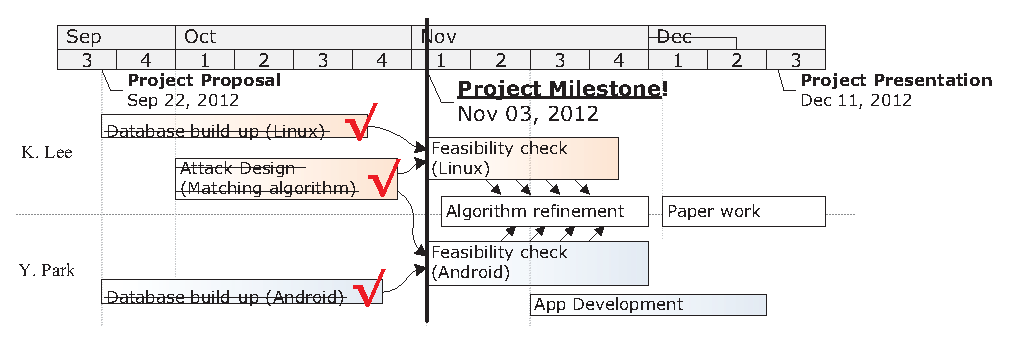
\includegraphics{Figures/Timeline_Mile}
\caption{Timeline}
\label{fig:timeline}
\vspace{-5mm}
\end{figure}